%\documentclass[preprints,article,accept,moreauthors,pdftex,10pt,a4paper]{Definitions/mdpi} 
%DIF LATEXDIFF DIFFERENCE FILE
%DIF DEL cpbe-submitted-draft.tex   Tue Aug 21 09:04:33 2018
%DIF ADD cpbe.tex                   Tue Aug 21 14:08:44 2018
\documentclass[arts,article,submit,moreauthors,pdftex,10pt,a4paper]{Definitions/mdpi} 

%=================================================================
\firstpage{1} 
\makeatletter 
\setcounter{page}{\@firstpage} 
\makeatother
\pubvolume{xx}
\issuenum{1}
\articlenumber{1}
\pubyear{2018}
\copyrightyear{2018}
\externaleditor{Academic Editor: name}
\history{Received: date; Accepted: date; Published: date}

%------------------------------------------------------------------
% The following line should be uncommented if the LaTeX file is uploaded to arXiv.org
%\pdfoutput=1

%\updates{yes} % If there is an update available, un-comment this line

%=================================================================
% Add packages and commands here. The following packages are loaded in our class file: fontenc, calc, indentfirst, fancyhdr, graphicx, lastpage, ifthen, lineno, float, amsmath, setspace, enumitem, mathpazo, booktabs, titlesec, etoolbox, amsthm, hyphenat, natbib, hyperref, footmisc, geometry, caption, url, mdframed, tabto, soul, multirow, microtype, tikz

\usepackage[utf8]{inputenc}

% Bibliography
%\usepackage[
%  backend=biber,
%  style=authoryear-icomp,
%  url=true
%]{biblatex}
%\addbibresource{references.bib}

%\usepackage[]{hyperref}
%\hypersetup{
%  colorlinks=true,
%}

% Colored outcome tags:
\definecolor{enables}{HTML}{00AADD}
\definecolor{threatens}{HTML}{DDAA00}
\definecolor{advances}{HTML}{0033AA}
\definecolor{hinders}{HTML}{991100}
\newcommand{\enables}{\textbf{\color{enables}enables}}
\newcommand{\advances}{\textbf{\color{advances}advances}}
\newcommand{\threatens}{\textbf{\color{threatens}threatens}}
\newcommand{\hinders}{\textbf{\color{hinders}hinders}}

\newcommand{\enablez}{\textbf{\color{enables}enable}}
\newcommand{\advancez}{\textbf{\color{advances}advance}}
\newcommand{\threatenz}{\textbf{\color{threatens}threaten}}
\newcommand{\hinderz}{\textbf{\color{hinders}hinder}}

%=================================================================
% Full title of the paper (Capitalized)
\Title{Choice Poetics by Example}

% Author Orchid ID: enter ID or remove command
\newcommand{\orcidauthorA}{0000-0001-7821-1973} % Use \orcidA{} below
\newcommand{\orcidauthorB}{0000-0003-3874-1720}
\newcommand{\orcidauthorC}{0000-0002-1897-6293}
\newcommand{\orcidauthorD}{0000-0003-1964-7624}

% Authors, for the paper (add full first names)
\Author{Peter Mawhorter *$^{1}$ \orcidA{}, Carmen Zegura $^{2}$, Alex Gray $^{3}$, Arnav Jhala $^{3}$ \orcidB{}, Michael Mateas $^{4}$ \orcidC{} and Noah Wardrip-Fruin $^{4}$ \orcidD{}}

% Authors, for metadata in PDF
\AuthorNames{Peter Mawhorter, Arnav Jhala, Michael Mateas and Noah Wardrip-Fruin}

% Affiliations / Addresses (Add [1] after \address if there is only one affiliation.)
\address{%
$^{1}$ \quad Massachusetts Institute of Technology; pmawhorter@gmail.com\\
$^{2}$ \quad Brown University; carmen\_zegura@brown.edu\\
$^{3}$ \quad North Carolina State University; [magray2, ajhala]@ncsu.edu\\
$^{4}$ \quad University of California Santa Cruz; [michaelm, nwf]@soe.ucsc.edu}

% Contact information of the corresponding author
\corres{Correspondence: pmawhorter@gmail.com}

\abstract{%
%DIF 83c83
%DIF < Choice poetics is a formalist framework that seeks to capture the impacts choices have on player experiences within narrative games.
%DIF -------
Choice poetics is a formalist framework that seeks to concretely describe the impacts choices have on player experiences within narrative games. %DIF > 
%DIF -------
%
Developed in part to support algorithmic generation of narrative choices, the theory includes a detailed analytical framework for understanding the impressions choice structures make by analyzing the relationships between options, outcomes, and player goals.
%
The theory also emphasizes the need to account for players' various modes of engagement, which vary both during play and between players.
%
%DIF 89c89
%DIF < In this work, we illustrate the non-computational application of choice poetics to the analysis of three different choices, in order to further develop the theory and make it more accessible to others.
%DIF -------
In this work, we illustrate the non-computational application of choice poetics to the analysis of two different games, in order to further develop the theory and make it more accessible to others. %DIF > 
%DIF -------
%
%DIF 91c91
%DIF < We focus first on analyzing so-called false choices in the game ``Mass Effect,'' and show how they actually provide meaningfully different outcomes for players who are utilizing certain modes of engagement.
%DIF -------
We focus first on using choice poetics to examine the central repeated choice in ``Undertale,'' and show how it can be used to contrast two different player types that will approach a choice differently. %DIF > 
%DIF -------
%
%DIF 93-95c93
%DIF < Second, we use choice poetics to examine the central repeated choice in ``Undertale,'' and show how it can be used to contrast two different player types that will approach a choice differently.
%DIF < %
%DIF < Finally, we give an example of fine-grained analysis using a choice from the game ``Papers Please,'' which breaks down options and their outcomes to illustrate how the choice pushes players towards complicity via the introduction of uncertainty.
%DIF -------
Finally, we give an example of fine-grained analysis using a choice from the game ``Papers, Please,'' which breaks down options and their outcomes to illustrate exactly how the choice pushes players towards complicity via the introduction of uncertainty. %DIF > 
%DIF -------
%
Through all of these examples, we hope to show the usefulness of choice poetics as a framework for understanding narrative choices, and to demonstrate concretely how one could productively apply it to choices `in the wild.'}  

\keyword{choice poetics; poetics; narrative games; choices; player goals; roleplay; complicity}
%DIF PREAMBLE EXTENSION ADDED BY LATEXDIFF
%DIF UNDERLINE PREAMBLE %DIF PREAMBLE
\RequirePackage[normalem]{ulem} %DIF PREAMBLE
\RequirePackage{color}\definecolor{RED}{rgb}{1,0,0}\definecolor{BLUE}{rgb}{0,0,1} %DIF PREAMBLE
\providecommand{\DIFadd}[1]{{\protect\color{blue}\uwave{#1}}} %DIF PREAMBLE
\providecommand{\DIFdel}[1]{{\protect\color{red}\sout{#1}}}                      %DIF PREAMBLE
%DIF SAFE PREAMBLE %DIF PREAMBLE
\providecommand{\DIFaddbegin}{} %DIF PREAMBLE
\providecommand{\DIFaddend}{} %DIF PREAMBLE
\providecommand{\DIFdelbegin}{} %DIF PREAMBLE
\providecommand{\DIFdelend}{} %DIF PREAMBLE
%DIF FLOATSAFE PREAMBLE %DIF PREAMBLE
\providecommand{\DIFaddFL}[1]{\DIFadd{#1}} %DIF PREAMBLE
\providecommand{\DIFdelFL}[1]{\DIFdel{#1}} %DIF PREAMBLE
\providecommand{\DIFaddbeginFL}{} %DIF PREAMBLE
\providecommand{\DIFaddendFL}{} %DIF PREAMBLE
\providecommand{\DIFdelbeginFL}{} %DIF PREAMBLE
\providecommand{\DIFdelendFL}{} %DIF PREAMBLE
%DIF END PREAMBLE EXTENSION ADDED BY LATEXDIFF

\begin{document}

\maketitle

\section{Introduction}

Originally developed in some of our prior work \citep{mawhorter2014towards,mawhorter2015intentionally,mawhorter2015generating,mawhorter2016artificial}, choice poetics is a formalist framework for understanding the impact of narrative choices on the player experience via their options, their outcomes, and how those relate to player goals.
%
Choice poetics was developed in order to be deployed in a generative system that produces narrative choices, as described in \citep{mawhorter2015generating,mawhorter2016artificial}.
%
However, the theory also supports human analysis, and the goal of this paper is to provide examples of that.
%
We hope that these examples not only demonstrate the use of the framework, but also meaningfully contribute to existing discussions of the choices that we analyze.


\label{sec:analysis_steps}
The formal process of choice poetic analysis, having been designed with operationalization in mind, is quite detailed, but it can be summarized in four steps \DIFaddbegin \DIFadd{(concrete examples of these steps are provided later on)}\DIFaddend :
\begin{enumerate}
  \item \textbf{Goal Analysis}: Consider the player's mode(s) of engagement (e.g., role play, power play, etc.), and observe or assume the set of goals that influences their decisions. For a specific analysis, defining one or more \DIFdelbegin \DIFdel{model players in terms of goal sets }\DIFdelend \DIFaddbegin \DIFadd{player models (as prioritized set(s) of goals) }\DIFaddend is often sufficient.
  \item \textbf{Likelihood Analysis}: Review the options offered at the choice \DIFdelbegin \DIFdel{in question}\DIFdelend \DIFaddbegin \DIFadd{being analyzed}\DIFaddend , and note the full range of outcomes that \DIFdelbegin \DIFdel{they suggest }\DIFdelend \DIFaddbegin \DIFadd{those options might suggest to the player}\DIFaddend , as well as the outcomes they actually produce. Also note how likely each suggested outcome seems to be.
  \item \textbf{Prospective Analysis}: Describe the impact of each \emph{suggested outcome} on each player goal. This gives an overall impression of how the choice will appear to the player as they encounter it, known as their \textbf{prospective impression}. \DIFdelbegin \DIFdel{Specific option}\DIFdelend \DIFaddbegin \DIFadd{Option}\DIFaddend /outcome patterns \DIFdelbegin \DIFdel{may be }\DIFdelend \DIFaddbegin \DIFadd{are }\DIFaddend recognizable at this point.
  \item \textbf{Retrospective Analysis}: Review the \emph{actual} outcomes of each option, and describe their impacts on each player goal. This produces a picture of the \textbf{retrospective impression} that the choice will leave on the player once they observe an outcome. Pay close attention to any differences between suggested and actual outcomes. Again, specific patterns may be identifiable at this stage.
\end{enumerate}
\DIFdelbegin \DIFdel{Usually, }\DIFdelend \DIFaddbegin \DIFadd{These four steps produce tables of prospective and retrospective impression labels for each option, which can usually be used to answer }\DIFaddend specific questions about a choice \DIFdelbegin \DIFdel{can be answered by examining the prospective and/or retrospective impression tables for each option at a choice}\DIFdelend \DIFaddbegin \DIFadd{(e.g., ``Which option will this type of player favor?'' or ``Will the player feel this is a difficult choice?'').
%DIF > 
In some cases, producing multiple contrasting analyses using different starting assumptions (such as about player goals or outcome likelihoods) can be used to answer design questions (e.g., ``Will this choice tend to separate players according to player types?'' or ``Should the likelihood of this outcome be important for how players will perceive this choice?'')}\DIFaddend .

\label{sec:prospective_labels}

For prospective analysis, the valence and likelihood of outcomes can be summarized using concise labels.
%
For each option $\times$ goal, labels can be assigned depending on whether that option has likely/unlikely outcomes that advance/hinder that goal.
%
For likely outcomes, we assign the labels \advances{} and \hinders{}, and for unlikely/unknown outcomes, we use the labels \enables{} and \threatens{}.
%
Note that most option/goal combinations will receive more than one label, e.g., an advantageous but not certain option could both \threatenz{} and \advancez{} a goal.
%
The assignment of prospective labels allows us to analyze the choice by comparing it to known choice structures, or just by observing patterns among the labels.


\DIFdelbegin \DIFdel{Our first example analysis is a ``false'' choice from the game }\emph{\DIFdel{Mass Effect}} %DIFAUXCMD
\DIFdel{\mbox{%DIFAUXCMD
\citep{bioware2007mass}}\hspace{0pt}%DIFAUXCMD
, which demonstrates the importance of modes of engagement in approaching choice analysis.
%DIF < 
Throughout the game, the player is presented with choices where several options lead to identical results, even to the point where the dialogue spoken by the player character as a result of the choice is the same.
%DIF < 
The motives behind these choice constructions and their impact on the player have already been discussed (see e.g., \mbox{%DIFAUXCMD
\cite{jorgensen2010game,bizzocchi2012mass,boyan2015massively}}\hspace{0pt}%DIFAUXCMD
), but we feel that their specific relation to role play has not been examined in detail.
%DIF < 
As we will demonstrate, a careful consideration of possible player goals reveals that these choices, which seem to have no difference in their outcomes, can actually have significance for the extra-digital narrative produced by the player, and they are thereby meaningful for players who are interested in role play.
}%DIFDELCMD < 

%DIFDELCMD < %%%
\DIFdel{After highlighting modes of engagement in }\emph{\DIFdel{Mass Effect}}%DIFAUXCMD
\DIFdel{, we give }\DIFdelend \DIFaddbegin \DIFadd{We start with }\DIFaddend an example of contrasting modes of engagement by looking at \emph{Undertale}'s central repeated choice of how to interact with wandering monsters \citep{fox2015undertale}.
%
\emph{Undertale}'s plot revolves around the player's aggression: does the player take their cue from other games and attack every `monster' they come across, or do they instead use the game's unusual `Mercy' option to avoid violence?
%
Our analysis of \emph{Undertale} examines both how that choice changes as the player learns about its outcomes, and how different goals might lead to different play styles.
%
The game reinforces both aggressive and pacifist styles but gives those players different endings to encourage dialogue within the player community.


After exploring the importance of modes of engagement, we shift focus by deconstructing a repeated choice from \emph{Papers\DIFaddbegin \DIFadd{, }\DIFaddend Please}: whether or not to approve the entry permit of someone who claims to be a refugee \citep{pope2013papers}.
%
\emph{Papers\DIFaddbegin \DIFadd{, }\DIFaddend Please} uses a carefully crafted choice structure to illustrate to the player how autocratic regimes instill complicity in their citizens by manipulating uncertainty.
%
A detailed analysis of the options and outcomes involved reveals exactly how this choice structure operates, and how it would take a different form without the element of uncertainty.
%
\DIFdelbegin \DIFdel{By putting the player in a situation in which they themselves become complicit, }\emph{\DIFdel{Papers Please}} %DIFAUXCMD
\DIFdel{leverages the full power of interactive media to evoke empathy via interactive perspective-taking}\DIFdelend \DIFaddbegin \DIFadd{Choice poetics is useful here because it can show explicitly how important uncertainty is to the effect achieved by }\emph{\DIFadd{Papers, Please}}\DIFadd{, illustrating not just that the game }\emph{\DIFadd{does}} \DIFadd{encourage complicity, but the subtle psychological mechanism it uses to do so}\DIFaddend .


By providing examples of the application of choice poetics ``by hand'' as opposed to algorithmically, we hope to inspire others to use and eventually help refine this theory.
%
Ideally, the formal structure of choice poetics can provide language to discuss choice structures precisely, and the exhaustive analysis of goals, options, and outcomes can help analysts uncover quirks and details not readily apparent from a more gestalt perspective.
%
Although we do not believe in formalism as an ultimate goal of literary (or interactive) analysis, we do hope that this framework can become one useful tool among many for both designers and critics to better understand the impacts of narrative choices on their audiences.

\section{Related Work}

\DIFdelbegin \DIFdel{As already mentioned, this }\DIFdelend \DIFaddbegin \DIFadd{This }\DIFaddend work builds on our previous work on the theory of choice poetics.
%
In particular, our paper ``Towards a Theory of Choice Poetics'' \citep{mawhorter2014towards} provides a concise summary of the aims of the theory and the phenomena that it attempts to explain, and Peter Mawhorter's dissertation \citeyear{mawhorter2016artificial} contains a chapter that provides a more detailed examination of the theory, including a walkthrough of the \emph{Papers\DIFaddbegin \DIFadd{, }\DIFaddend Please} example that we also present here.
%
It is worth acknowledging the lines of inquiry that choice poetics is in dialogue with, including formalist narratology (from Aritstotle \citeyear{aristotle1917poetics} to Barthes \citeyear{barthes1975introduction}), the psychology of narrative \citep{tversky1981framing,green2000role,mar2008function,zunshine2006why}, the psychology of decision-making \citep{mellers1997decision,schwartz2002maximizing}, and of course other modern theories of interactive narrative \citep{aarseth1997cybertext,murray1997hamlet,ryan1991possible,tosca2000pragmatics,mateas2001preliminary,frasca2003ludologists,lindley2005story}.
%
The \DIFaddbegin \DIFadd{specific ideas about modes of engagement and player motivations used here are based largely on the work of Yee \mbox{%DIFAUXCMD
\citeyear{yee2006motivations}}\hspace{0pt}%DIFAUXCMD
, along with other work summarized in \mbox{%DIFAUXCMD
\citep{hamari2014player}}\hspace{0pt}%DIFAUXCMD
, although choice poetics can also incorporate non-standard modes of engagement such as critical play \mbox{%DIFAUXCMD
\citep{flanagan2009critical} }\hspace{0pt}%DIFAUXCMD
(see Chapter 3 of \mbox{%DIFAUXCMD
\citep{mawhorter2016artificial} }\hspace{0pt}%DIFAUXCMD
for a more detailed explanation of these links).
%DIF > 
Other relevant studies provide insight into how engagement can be driven by multiple desires \mbox{%DIFAUXCMD
\citep{lindley2005story}}\hspace{0pt}%DIFAUXCMD
, can be affected by choices and their consequences \mbox{%DIFAUXCMD
\citep{mallon2005stand}}\hspace{0pt}%DIFAUXCMD
, and can change over time \mbox{%DIFAUXCMD
\citep{lange2014youre}}\hspace{0pt}%DIFAUXCMD
.
%DIF > 
The }\DIFaddend development of choice poetics was also informed by non-academic writing on choice design, such as design advice for authors of online interactive narratives \citep{choiceofgames2010rules} or tabletop roleplaying game masters \citep{laws2001robin}.
%
Finally, concurrent experimental work (including some of our own) around choices and outcomes in games has provided useful empirical data about choices and their consequences \citep{fendt2012achieving,cardonarivera2014foreseeing,mawhorter2015generating,iten2018choosing}.
%DIF < 
\DIFdelbegin \DIFdel{In the context of our present analysis, it is useful to also discuss existing theoretical treatments of the specific choice types under consideration.
}\DIFdelend 


\DIFdelbegin %DIFDELCMD < \subsection{False Choices}
%DIFDELCMD < 

%DIFDELCMD < %%%
\DIFdel{The subject of false choices in games has already received serious critical and scholarly attention.
%DIF < 
For instance, the }\emph{\DIFdel{Extra Credits}} %DIFAUXCMD
\DIFdel{video series (which focuses on games criticism for a popular audience) has discussed false choices, and even used }\emph{\DIFdel{Mass Effect}} %DIFAUXCMD
\DIFdel{as an example \mbox{%DIFAUXCMD
\citep{floyd2013illusion}}\hspace{0pt}%DIFAUXCMD
.
%DIF < 
Their analysis focuses on the necessity of false choice as a means of avoiding budget problems due to content expansion, but our analysis emphasizes the fact that these choices are not completely illusory, at least for certain players.
%DIF < 
As already mentioned, scholarly studies of }\emph{\DIFdel{Mass Effect}} %DIFAUXCMD
\DIFdel{have also touched upon the subject:
}%DIFDELCMD < \begin{itemize}
\begin{itemize}%DIFAUXCMD
%DIFDELCMD <   \item %%%
\item%DIFAUXCMD
\DIFdel{In ``Game Characters as Narrative Devices. }%DIFDELCMD < {%%%
\DIFdel{A}%DIFDELCMD < } %%%
\DIFdel{Comparative Analysis of }\emph{\DIFdel{Dragon Age: Origins}} %DIFAUXCMD
\DIFdel{and }\emph{\DIFdel{Mass Effect 2}}%DIFAUXCMD
\DIFdel{,'' Kristine J}%DIFDELCMD < {%%%
\DIFdel{\o}%DIFDELCMD < }%%%
\DIFdel{rgensen (\mbox{%DIFAUXCMD
\citeyear{jorgensen2010game}}\hspace{0pt}%DIFAUXCMD
) discusses role play in }\emph{\DIFdel{Mass Effect 2}} %DIFAUXCMD
\DIFdel{and mentions the limited agency given to the player. They can shape the main character's actions to a degree, but don't have full control over the end result, in part because of discrepancies between player-selected text and the voice-acted outcomes that result. The resulting distance between character and player is something that players who are interested in full control over the construction of their character's persona might want to erase, and we argue here that seemingly inconsequential choices can give the player some room to do so.
  }%DIFDELCMD < \item %%%
\item%DIFAUXCMD
\DIFdel{In ``}\emph{\DIFdel{Mass Effect 2}}%DIFAUXCMD
\DIFdel{: A Case Study in the Design of Game Narrative,'' Jim Bizzocchi and Joshua Tanenbaum (\mbox{%DIFAUXCMD
\citeyear{bizzocchi2012mass}}\hspace{0pt}%DIFAUXCMD
) discuss several playthroughs of }\emph{\DIFdel{Mass Effect 2}}%DIFAUXCMD
\DIFdel{, and give a detailed account of their experiences. They also briefly mention false choices, as well as the fact that the main character has certain qualities that are outside the player's control.
}
\end{itemize}%DIFAUXCMD
%DIFDELCMD < \end{itemize}
%DIFDELCMD < 

%DIFDELCMD < %%%
\DIFdel{Other work not related to }\emph{\DIFdel{Mass Effect}} %DIFAUXCMD
\DIFdel{has also discussed the impacts of choices and how these affect the player.
%DIF < 
For example, Anders Tychsen and Michael Hitchens have talked about how consequences are managed in the shared narrative worlds of multiplayer online games \mbox{%DIFAUXCMD
\citep{tychsen2006ghost}}\hspace{0pt}%DIFAUXCMD
, and Richard Andrews has explained in detail how }\emph{\DIFdel{The Stanley Parable}} %DIFAUXCMD
\DIFdel{is ultimately about the constructed nature of choices in games and how that inevitably limits the player's agency \mbox{%DIFAUXCMD
\citep{andrews2017metagames}}\hspace{0pt}%DIFAUXCMD
.
%DIF < 
Gail Carmichael and David Mould have grappled with how player choice can be reconciled with nonlinear narrative techniques, and discuss different levels of playability; a useful framework for thinking about }\emph{\DIFdel{Mass Effect}}%DIFAUXCMD
\DIFdel{'s choices \mbox{%DIFAUXCMD
\citep{carmichael2014chronologically}}\hspace{0pt}%DIFAUXCMD
.
}%DIFDELCMD < 

%DIFDELCMD < %%%
\DIFdel{Because our take on }\emph{\DIFdel{Mass Effect}}%DIFAUXCMD
\DIFdel{'s choices is that they matter to some players but not others, it is also important to mention previous work on modes of engagement with games.
%DIF < 
Craig Lindley has an excellent treatment of some of these modes, and discusses the different pleasures of being a passive audience member, an active performer, and a completely immersed player \mbox{%DIFAUXCMD
\citep{lindley2005story}}\hspace{0pt}%DIFAUXCMD
.
%DIF < 
In particular, Lindley's performer mode of engagement specifically addresses the pleasures of performance that we claim are affected by the ``false'' choices in }\emph{\DIFdel{Mass Effect}}%DIFAUXCMD
\DIFdel{.
%DIF < 
Interestingly enough, empirical studies of player behavior suggest that while people who explicitly role-play are probably not a majority \mbox{%DIFAUXCMD
\citep{lange2014youre}}\hspace{0pt}%DIFAUXCMD
, many do still enjoy interactions related to characterization in narrative games (\mbox{%DIFAUXCMD
\cite{mallon2005stand}}\hspace{0pt}%DIFAUXCMD
, see especially pp. 6--7).
}%DIFDELCMD < 

%DIFDELCMD < %%%
\DIFdelend \subsection{Moral Choices}

Our \DIFdelbegin \DIFdel{second }\DIFdelend \DIFaddbegin \DIFadd{first }\DIFaddend analysis engages with the popular 2015 indie roleplaying game \emph{Undertale} and how players with similar goals but different priorities can be steered towards different decisions.
%
Existing scholarly literature on \emph{Undertale} has examined its portrayal of morality and ethics through its primary choice of 'kill' or 'spare' \citep{muller2017undertale}, the ways the game solidifies the significance of its choices through various mechanics \citep{day2017agency}, and how its musical score changes from tonal and pleasant to atonal and eerie depending on the player's approach \citep{perez2017undertale}.
%
Notably, \emph{Undertale} goes so far as to remember a player's decisions even after they ostensibly reset the game, encouraging the idea that its choices are meaningful \citep{hughes2015undertale}.
%
Although \emph{Undertale}'s designer Toby Fox has been reticent about his intentions regarding the game's moral choices, he is clearly interested in aspects of game design beyond traditional roleplaying game mechanics (quoted in \cite{feeld2015interview}):

\begin{quote}
  \itshape
The addictive quality of ``numbers increasing'' is what drives a lot of games. But some of the most important things in life can't be accurately represented by numbers.
\end{quote}


\DIFaddbegin \DIFadd{As described by Müller, Undertale's various endings have encouraged the player community to discuss attitudes towards violence both in games and in real life (\mbox{%DIFAUXCMD
\cite{muller2017undertale}}\hspace{0pt}%DIFAUXCMD
, §2.2.1).
%DIF > 
The usefulness of choice poetics in this context is that is provides a concrete way of describing which aspects of Undertale's central kill/spare choice are mobilized to achieve this result, and by contrasting two different possible player perspectives, it illustrates how different players might naturally be encouraged to pursue different play styles and therefore observe different content, providing fodder for online discussion.
%DIF > 
Of course, a formalist analysis is not the only way to reach that conclusion, but it is a mechanical and reproducible way to do so, potentially making it accessible to novice critics (and as in our prior work, to automated systems).
}


\DIFaddend Broader research on moral choices in games includes examinations of their implementation and studies of how players respond to them \citep{svelch2010good,weaver2012mirrored,consalvo2016playing}.
%
Of course, research on the psychological effects of games, especially violent games, is quite popular, but has come to largely mixed conclusions \citep{ferguson2008school,ellithorpe2015moral}.
%
In fact, there is also interest in using video games to encourage better moral decision making \citep{kastarov2017training}\DIFaddbegin \DIFadd{.
}\DIFaddend 


\subsection{Coercion and Complicity}

In our \DIFdelbegin \DIFdel{third }\DIFdelend \DIFaddbegin \DIFadd{second }\DIFaddend example analysis, we will discuss complicity in \emph{Papers\DIFaddbegin \DIFadd{, }\DIFaddend Please}, and use a detailed breakdown of a single choice to illustrate how this moral issue is raised within the game.
%
A version of this analysis appears in \citep{mawhorter2016artificial}, but a more thorough analysis of the game and its themes has also been undertaken by 
Paul Formosa, Malcolm Ryan, and Dan Staines (\citeyear{formosa2016papers}; for a critical perspective, see also \cite{alexander2013designing}, which Formosa et al. cite themselves).
%
Formosa, Ryan, and \DIFdelbegin \DIFdel{Stanies}\DIFdelend \DIFaddbegin \DIFadd{Staines}\DIFaddend ' excellent analysis of the game and its relationship with morality largely agrees with our conclusion that the game uses ambiguity as a mechanism to encourage complicity, and in fact they even quote personal correspondence with Lucas Pope, the game's designer, to the same effect: ``On some level I want players to reach a point of self-realization---about how good people can be turned into uncaring cogs,'' (Pope quoted in \cite{formosa2016papers}).
%
We \DIFdelbegin \DIFdel{believe that the choice poetics approach to analysis is useful not because it can reach the same conclusions as others, but because it can give a }\DIFdelend \DIFaddbegin \DIFadd{find these congruences encouraging, because they show that choice poetics can produce conclusions that are not only echoed by other analyses but which also seem to have been intended by the designer themselves.
%DIF > 
Of course, if existing analyses have reached these conclusions already, why use choice poetics at all?
%DIF > 
In this case, choice poetics provides a more }\DIFaddend detailed accounting of \DIFdelbegin \DIFdel{why a particular choice operates in the way it does, and from a designer}\DIFdelend \DIFaddbegin \DIFadd{the importance of ambiguity in terms of the choices faced by the player, and is able to explain exactly why removing ambiguity would change a (hypothetical) player}\DIFaddend 's perspective \DIFdelbegin \DIFdel{, may offer insight about what to tweak to change the player experience}\DIFdelend \DIFaddbegin \DIFadd{on the game.
%DIF > 
Such detailed accounting of the impact of outcomes could be useful for designers interested in tweaking their choices to best support desired narrative or persuasive goals, and in fact, at least for machine-designed choices, this has shown to be somewhat effective (see \mbox{%DIFAUXCMD
\cite{mawhorter2015intentionally}}\hspace{0pt}%DIFAUXCMD
)}\DIFaddend .



Beyond analyses of \emph{Papers\DIFaddbegin \DIFadd{, }\DIFaddend Please}, other scholarly work dealing with complicity in games is relevant here.
%
Toby Smethurst and Stef Craps have discussed the appearance of trauma in games, including a section on complicity \citep{smethurst2015playing}.
%
\DIFdelbegin \DIFdel{Their work is also relevant to our analysis of }\emph{\DIFdel{Mass Effect}} %DIFAUXCMD
\DIFdel{because they discuss role-playing and false choices.
%DIF < 
}\DIFdelend In a similar vein, Holger Pötzsch has discussed complicity in games, again in the context of more scripted narrative settings \citep{potzsch2017selective}.
%
Both of these analyses include \emph{Spec Ops: The Line} \citep{yager2012spec} as an example of a game that deals with complicity, but \DIFdelbegin \DIFdel{it }\DIFdelend \DIFaddbegin \DIFadd{which }\DIFaddend does so in a completely different manner to \emph{Papers\DIFaddbegin \DIFadd{, }\DIFaddend Please}, using a scripted narrative and being much more direct and extreme about the moral decisions being made (see also \cite{murray2016race} on the game's failure to grapple with issues of racism and sexism even as it does address toxic masculinity).


\DIFdelbegin %DIFDELCMD < \section{``False'' Choices in \emph{Mass Effect}}
%DIFDELCMD < 

%DIFDELCMD < %%%
\DIFdel{The first step in any choice poetic analysis is determining the motivations and goals of the player(s) you want to consider.
%DIF < 
Generally, there will be multiple player types who will engage differently with a choice under consideration, and identifying these player types (or even just limiting analysis to a single type for expedience) is a prerequisite for detailed choice analysis.
%DIF < 
False choices in }\emph{\DIFdel{Mass Effect}} %DIFAUXCMD
\DIFdel{help to illustrate why these considerations are so important, because despite having no }\emph{\DIFdel{systemic}} %DIFAUXCMD
\DIFdel{consequences within the game, they offer opportunities for the player to flesh out their own version of the main character who has specific mannerisms and preferences.
%DIF < 
For players interested in engaging with the game as role players, especially those who want to act out a specific persona, these ``false'' choice have real consequences.
}%DIFDELCMD < 

%DIFDELCMD < %%%
\DIFdel{For a detailed description of }\emph{\DIFdel{Mass Effect}} %DIFAUXCMD
\DIFdel{gameplay (largely the same between different games in the trilogy), we invite the reader to consult \mbox{%DIFAUXCMD
\cite{bizzocchi2012mass}}\hspace{0pt}%DIFAUXCMD
.
%DIF < 
For our purposes, it suffices to note that within a science fiction universe, the player is thrust into the role of Commander Shepard, the protagonist in a galactic struggle to unite several alien factions against a formidable and ancient threat.
%DIF < 
Although the player may choose a first name, the outline of a backstory, and a profession for Shepard, the character has some distinctive qualities that the player cannot really alter: Shepard will always be a commander, and will take an active role in the events that unfold.
}%DIFDELCMD < 

%DIFDELCMD < %%%
\DIFdel{Throughout the game, interactions with other characters are carried out via dialogue trees, where options are selected from a wheel of responses.
%DIF < 
Fig. \ref{fig:ME_false} shows an example of this interface, and also illustrates the most extreme version of a false choice---in the choice shown, all three text options lead to exactly the same spoken response (and they have no other consequences within the game later)}\footnote{\DIFdel{A video that gives more context for this choice and which shows the responses to different choices throughout this scene is available at: }%DIFDELCMD < \url{https://www.youtube.com/watch?v=8BewZnUnDoE}%%%
}%DIFAUXCMD
\addtocounter{footnote}{-1}%DIFAUXCMD
\DIFdel{.
%DIF < 
As with most choices in the game, none of the text responses exactly matches the spoken dialogue, and this serves not only to obfuscate false choices like this one but also to position the text choices as something closer to a character's internal monologue than an external diegetic utterance.
%DIF < 
Thinking of the option text in this way reveals that although these choices may not have consequences within the game, they do lead to different portrayals of Shepard's character.
%DIF < 
When faced with stonewalling from the council bureaucracy, who in this case are denying his eyewitness testimony against a traitorous special agent, is Shepard the kind of person who is defiant, or resigned?
}%DIFDELCMD < 

%DIFDELCMD < %%%
\DIFdel{The spoken response is cleverly crafted so that it can be read in multiple ways.
%DIF < 
If you selected ``You won't see the truth,'' Shepard's utterance seems to take on more defiant undertones than if you selected ``What's the point?'' even though the delivery is identical.
%DIF < 
And although within the mechanical systems of the game this choice has no consequences, Shepard's attitude is an important part of who they are, so for someone interested in crafting a specific narrative that portrays Shepard in a particular light (as e.g., \mbox{%DIFAUXCMD
\cite{bizzocchi2012mass} }\hspace{0pt}%DIFAUXCMD
did in their close playing of }\emph{\DIFdel{Mass Effect 2}}%DIFAUXCMD
\DIFdel{), the nuances of these responses have consequences for that portrayal.
%DIF < 
Over the course of the game, the way that many ``false'' choices are made can add up to redefine the character enacted by the player, and since in many cases some choices along a particular axis (such as the defiant--resigned range suggested here) will have more serious in-game consequences, not all of them need to in order to have meaning to the player.
}%DIFDELCMD < 

%DIFDELCMD < %%%
\DIFdel{To draw this same conclusion by another process, we can observe that even at the player-goal estimation stage of choice poetics analysis, it becomes clear that any mechanics-related considerations regarding this choice will be irrelevant, because it produces no distinct in-game outcomes.
%DIF < 
If an analyst were to consider this choice using a set of diegetic player goals, they would rightly conclude that although the options presented might }\emph{\DIFdel{suggest}} %DIFAUXCMD
\DIFdel{some relevance (e.g., to a goal of pleasing the council members), the outcome, due to being singular, does not actually have any.
%DIF < 
However, such an analytical outcome should naturally provoke the question: ``For what set of player goals }\emph{\DIFdel{would}} %DIFAUXCMD
\DIFdel{this choice have different outcomes?''---to which the answer is exactly: a set of player goals which includes preferences over not only in-game outcomes but also external considerations, such as the story that the player helps to express through their gameplay.
}%DIFDELCMD < 

%DIFDELCMD < %%%
\DIFdel{Even the partial lists of modes of engagement that have been suggested for choice poetics (see e.g., \mbox{%DIFAUXCMD
\cite{mawhorter2014towards}}\hspace{0pt}%DIFAUXCMD
) include role play as an important player perspective, and that is at least one perspective which includes goals involving the narrative produced by gameplay, rather than simply goals described in terms of the game's mechanics alone.
%DIF < 
Once we begin to consider such goals, we have to take a different view of options and outcomes as well.
%DIF < 
Whereas an initial analysis might label a choice as having only one outcome no matter the option selected, a more nuanced analysis would consider divergent portrayals of Shepard's character as divergent outcomes, with their own relationships with various possible player goals.
%DIF < 
The result of this line of reasoning is the realization that even the illusion of choice can have consequences for players who value the impressions their play creates.
}%DIFDELCMD < 

%DIFDELCMD < \begin{figure}
%DIFDELCMD <   
\includegraphics[width=0.5\textwidth]{fig/anything_else_to_add_1.png}
%DIFDELCMD <   
\includegraphics[width=0.5\textwidth]{fig/made_your_decision_1.png}
%DIFDELCMD <   %%%
%DIFDELCMD < \caption{%
{%DIFAUXCMD
\DIFdelFL{Two screenshots from }\emph{\DIFdelFL{Mass Effect}} %DIFAUXCMD
\DIFdelFL{showing the moment before and after making a choice. An NPC asks ``Do you have anything else to add, Commander Shepard?'' and the options given are labeled ``You won't see the truth,'' ``No,'' and ``What's the point?'' No matter which option you select, your character responds to the NPC with ``You've made your decision. I won't waste my breath.''}}
  %DIFAUXCMD
%DIFDELCMD < \label{fig:ME_false}
%DIFDELCMD < \end{figure}
%DIFDELCMD < 

%DIFDELCMD < %%%
\DIFdel{Although this conclusion may be apparent without resorting to a formal analysis of the choice in question, it highlights the importance of considering modes of engagement and player goals before analyzing a choice, and forced consideration of these factors tends to expose details like those explored here.
%DIF < 
It may also seem ridiculous to focus so much analytical effort on a single choice in a now decade-old game, but the broader implications of this line of reasoning should be of interest to designers.
%DIF < 
Rather than viewing such false choices as an evil necessitated by budgetary constraints, they can be thought of instead as opportunities to let the player develop their character in ways outside of the capabilities of whatever character modelling systems a game may contain.
%DIF < 
After all, }\emph{\DIFdel{Mass Effect}} %DIFAUXCMD
\DIFdel{has an entire subsystem dedicated to tracking a player's ``paragon'' and ``renegade'' points and attaching consequences to their actions along one dimension of behavior, but this choice does not engage with that system directly.
%DIF < 
Instead, choices such as this allow the player the opportunity to develop their character along a multitude of psychological dimensions without the designers having to implement systems for all of those.
}%DIFDELCMD < 

%DIFDELCMD < %%%
\DIFdelend \section{Reinforcing Disparate Choices in \emph{Undertale}}

\emph{Undertale} is an independently developed roleplaying game \citep{fox2015undertale} about a kid trying to get back home.
%
The game appears at first to be a normal roleplaying game with some interesting mechanics, but the facade of standard RPG mechanics hides a deeper morality-based storyline which challenges gamers to think more deeply about the random `monsters' they are fighting.
%
Players face different challenges and receive different endings depending on whether they play the game passively or aggressively.
%
These paths allow for the game to be a straightforward example of what happens when players with different play styles are forced to make the same choice.

\begin{figure}[t]
  \centering
    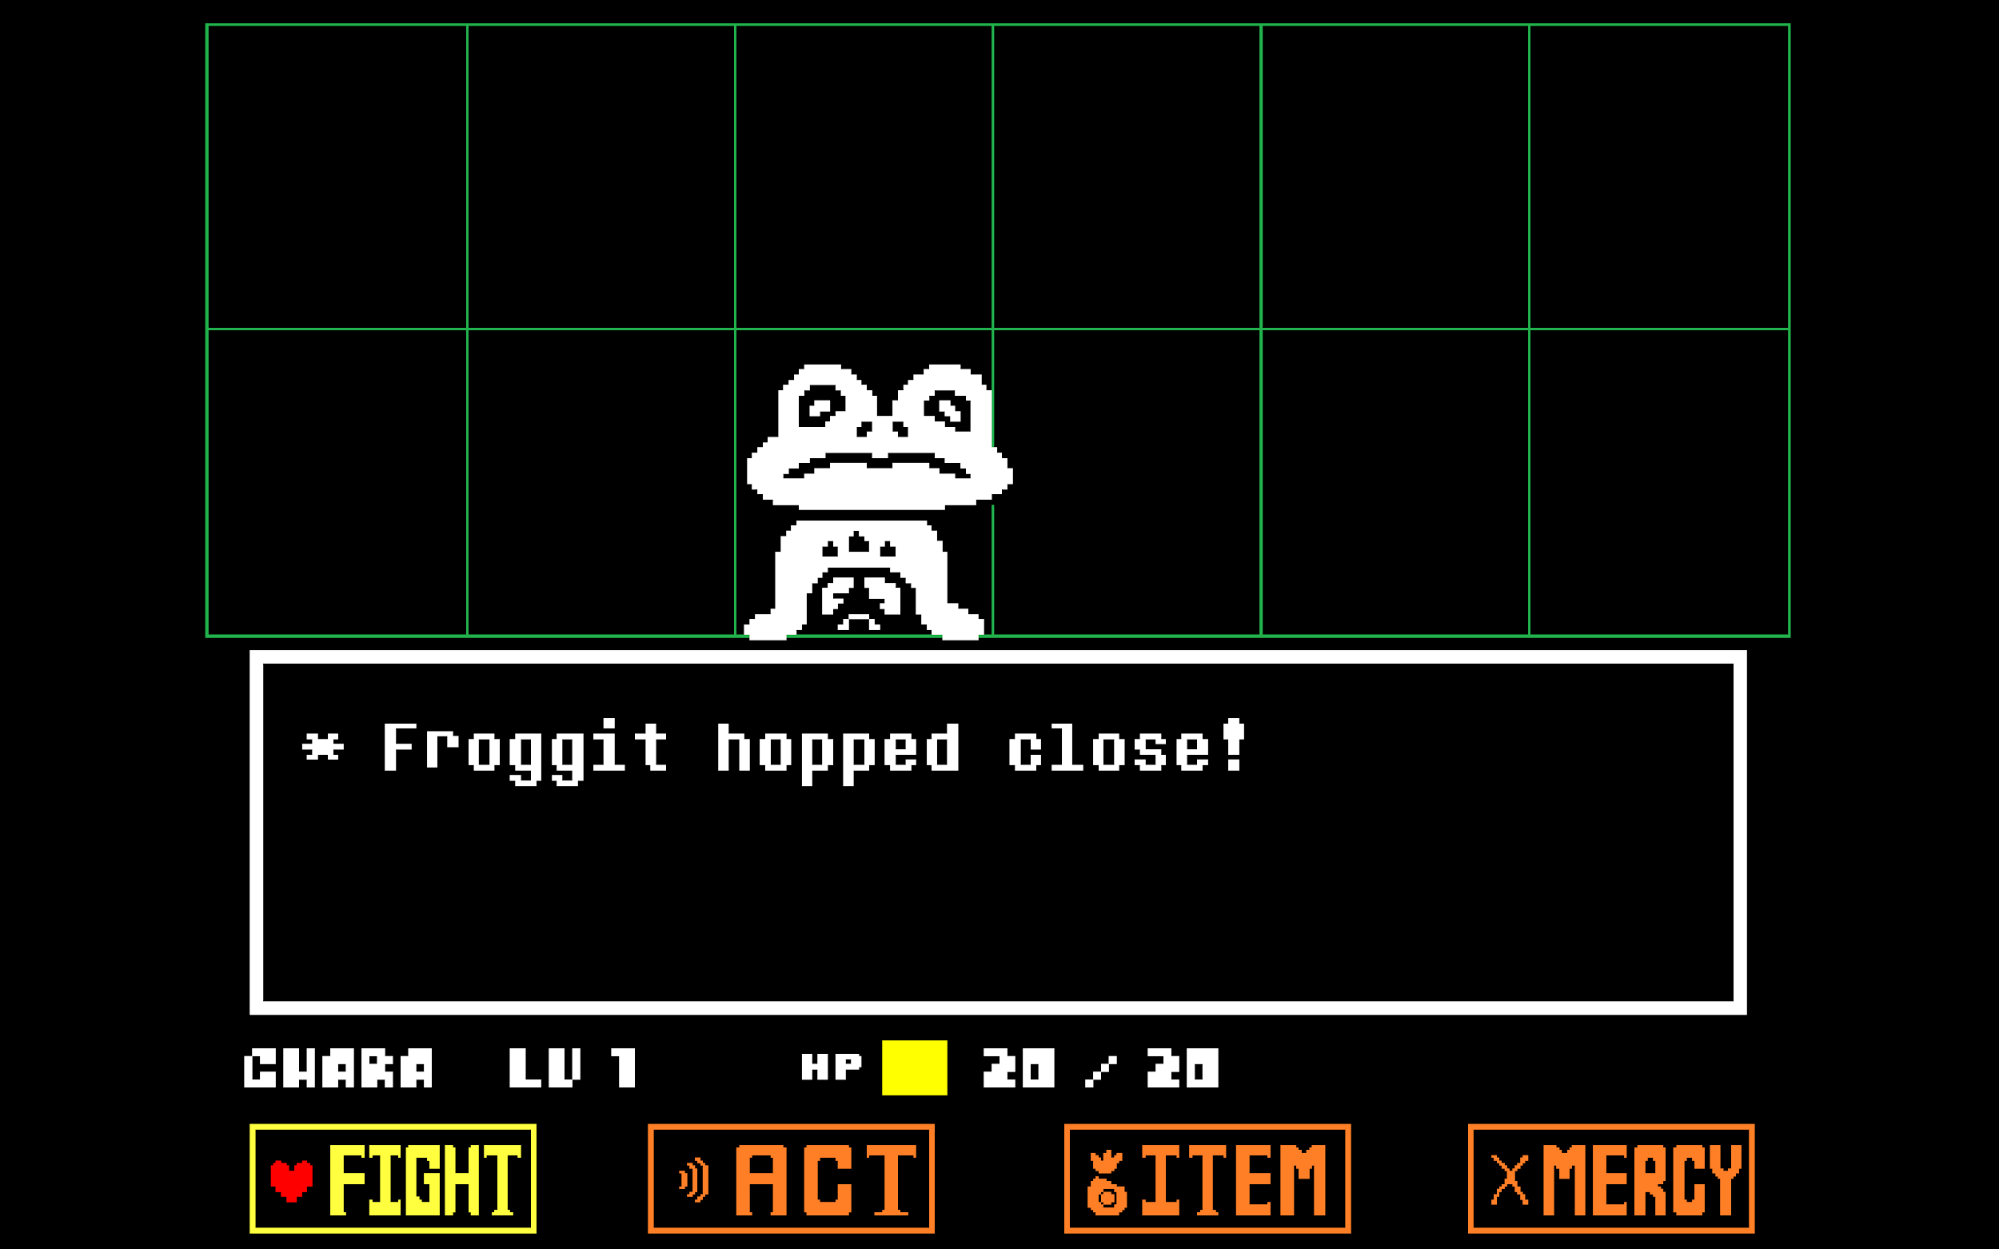
\includegraphics[width=0.8\textwidth]{fig/froggit.png}
    \caption{A screenshot from \emph{Undertale} showing the first random encounter of the game, in which a `Froggit' ``hops close,'' (note that aggression is implied via the convention of a random encounter but not \DIFdelbeginFL \DIFdelFL{via }\DIFdelendFL \DIFaddbeginFL \DIFaddFL{by }\DIFaddendFL the \DIFdelbeginFL \DIFdelFL{game's }\DIFdelendFL text). The \DIFdelbeginFL \DIFdelFL{main }\DIFdelendFL options are ``fight,'' ``act,'' ``item,'' and ``mercy,'' the last of which is unconventional.}
    \label{fig:UT_froggit}
\end{figure}

Figure \ref{fig:UT_froggit} shows the very first random encounter of the game, and illustrates the repeated central choice of whether to fight, flee, or `spare' each opponent (``Flee'' and ``Spare'' are the options in the ``Mercy'' menu).
%
With the exception of certain bosses, all `enemies' in the game must be dealt with in one of these three ways, where killing them awards gold and experience points, fleeing gives no reward, and sparing them awards just gold, \DIFdelbegin \DIFdel{and }\DIFdelend \DIFaddbegin \DIFadd{which }\DIFaddend is only possible after taking a specific sequence of actions that pacify the opponent which the player must learn for each type of `monster.'
%
To understand how this repeated choice is set up to create dialogue within player communities, we can break it down using a formal analysis.


To simplify the analysis somewhat, we ignore concerns about player skill, which would provide \DIFdelbegin \DIFdel{a }\DIFdelend \DIFaddbegin \DIFadd{an extra }\DIFaddend motive to select the `flee' option.
%
Although contrasting approaches to this choice across players of different skill levels would also be an interesting approach, we consider here the perspective of players that have no trouble with the challenges involved in either attacking or pacifying the enemies.


The remaining subsections here describe the results of each of the analysis steps outlined in section \ref{sec:analysis_steps}, and how they differ both for two different \DIFdelbegin \DIFdel{model players }\DIFdelend \DIFaddbegin \DIFadd{player models }\DIFaddend and between initial and subsequent encounters with the choice.
%
Our first \DIFdelbegin \DIFdel{model player }\DIFdelend \DIFaddbegin \DIFadd{player model}\footnote{\DIFadd{In choice poetics, a player model is defined as a specific set of prioritized goals, which makes it more specific than a `player type' as used in other literature, although our player models in this analysis roughly correspond to two popular `player types' identified in the literature (see below).}} \DIFaddend (we'll call them the power player) is \DIFaddbegin \DIFadd{intended to model }\DIFaddend an experienced roleplaying game player, who is familiar with the conventions of the genre and who expects to be asked to fight their way to victory, collecting experience and gold along the way to gain power and overcome challenging bosses.
%
\DIFdelbegin \DIFdel{Our second model player }\DIFdelend \DIFaddbegin \DIFadd{This power player model is grounded in the `Achievement' dimension of player motivation identified in \mbox{%DIFAUXCMD
\citep{hamari2014player}}\hspace{0pt}%DIFAUXCMD
, which corresponds to the idea of `power play' as a mode of engagement \mbox{%DIFAUXCMD
\citep{mawhorter2014towards}}\hspace{0pt}%DIFAUXCMD
.
%DIF > 
Our second player model }\DIFaddend (we'll call them the story player) \DIFdelbegin \DIFdel{is }\DIFdelend \DIFaddbegin \DIFadd{attempts to approximate }\DIFaddend someone who has little experience with roleplaying games and is interested in experiencing the story of \emph{Undertale}.
%
\DIFdelbegin \DIFdel{In terms of modes of engagement (cf. \mbox{%DIFAUXCMD
\cite{mawhorter2014towards}}\hspace{0pt}%DIFAUXCMD
),these model players are focused on power play and avatar play respectively}\DIFdelend \DIFaddbegin \DIFadd{This model is related to the dimension of player motivation that Hamari and Tuunanen identify as `Immersion,' and the `avatar play' mode of engagement from \mbox{%DIFAUXCMD
\citep{mawhorter2014towards}}\hspace{0pt}%DIFAUXCMD
}\DIFaddend .

\subsection{Goal Analysis}

We use the following set of goals, with the listed power/story priorities for our respective player models \DIFaddbegin \DIFadd{(these prioritized goal sets }\emph{\DIFadd{are}} \DIFadd{the player models)}\DIFaddend :

\begin{itemize}
  \item Gain experience points (high/low)---The power player prioritizes experience points (XP), knowing that they may be necessary to accumulate power and beat the game. The story player understands them as a reward, but does not seek them out to the detriment of other goals.
  \item Gain gold (high/low)---Just like XP, the power player seeks out gold while the story player welcomes it but does not prioritize it.
  \item Show mercy (none/high)---While the power player sees interactions with the monsters as instrumental and inconsequential, our hypothetical story player, swayed by the aesthetics of the game, finds them cute and feels bad being violent towards them (of course, not all story-focused players would have this outlook).
  \item Explore options (low/high)---Faced with a new game, both the power and story players are interested in figuring out what makes this game unique and what is possible within it, although for the power player this is secondary to other concerns. The `Mercy' menu especially, as an unconventional option, will attract interest.
  \item Behave consistently (low/low)---Both of our hypothetical players not only exhibit standard human biases towards consistent action (and justification of their past actions using future actions), but also recognize that in most game systems, rewards are reserved for extreme behavioral profiles. This goal does not trump others, but influences ambiguous cases.
\end{itemize}
Although these exact goal sets might not be those of \DIFdelbegin \DIFdel{real players, they serve our purpose of illuminating }\emph{\DIFdel{Undertale}}%DIFAUXCMD
\DIFdel{' s choice poetics.
}\DIFdelend \DIFaddbegin \DIFadd{any actual player, they do approximate common aspects of player psychology described within existing literature (e.g., the `Achievement' and `Immersion' dimensions from \mbox{%DIFAUXCMD
\cite{hamari2014player}}\hspace{0pt}%DIFAUXCMD
).
%DIF > 
Any concerns about particular goals or their prioritization could always be investigated by contrasting results with yet another player model that differed from one of these in terms of the goal in question, and of course, were data on actual player goals available in some form, it could be used to define detailed player models for personalized or aggregate analysis.
%DIF > 
Examples of blind playthroughs uploaded to YouTube (e.g., \mbox{%DIFAUXCMD
\cite{fuandon2015lets} }\hspace{0pt}%DIFAUXCMD
for the story player model and \mbox{%DIFAUXCMD
\cite{therpgminx2015lets} }\hspace{0pt}%DIFAUXCMD
for the power player model) also support the idea that these profiles might model some actual players.
}\DIFaddend 

\begin{table}[H]
\centering
\begin{tabular}{l l l}
  \toprule
 \multicolumn{1}{c}{\textbf{Fight}} & \multicolumn{1}{c}{\textbf{Flee}} & \multicolumn{1}{c}{\textbf{Spare}} \\
  \midrule
 (likely) Froggit dies & (likely) Froggit lives & (likely) Froggit lives \\
 (likely) XP reward & (likely) no XP & (unlikely) XP reward \\
 (likely) Gold reward & (likely) no Gold & (unlikely) Gold reward \\
 (known) New option & (known) New option & (known) New option \\
 (known) Not repeated & (known) Not repeated & (known) Not repeated \\
  \bottomrule
\end{tabular}
  \caption[\emph{Undertale} likelihood analysis]{Likelihood analysis for the player's initial encounter with the choice shown in Fig. \ref{fig:UT_froggit}. The ``new option'' `outcome' reflects the player goal of exploring unknown options, whereas the ``repeated'' `outcome' reflects the player goal of behaving consistently (both are the same for all three options the first time the player encounters this choice).}
\label{tab:UT_likelihoods}
\end{table}

\subsection{Likelihood Analysis}

The next task is to decide which options suggest what outcomes\DIFdelbegin \DIFdel{.
%DIF < 
Per our earlier examination of false choices, this }\DIFdelend \DIFaddbegin \DIFadd{, which }\DIFaddend can be tricky, as there is a wide range of possible outcomes to consider.
%
Luckily, our choice of player goals can narrow that range somewhat---for example, in this analysis, we have assumed our players are skilled enough that they will always succeed, so we ignore outcomes related to player injury or death.


Table \ref{tab:UT_likelihoods} shows likelihood analysis results for the player's first encounter with this choice (which are the same for both player models), including extradiegetic outcomes relating to exploration and consistency goals.
%
Once the player learns the actual outcomes of each choice, these likelihoods will be simplified: the player will know the true outcomes (all `likely' outcomes become `known'), and the two unlikely outcomes will be revealed (sparing rewards gold, but no XP).
%
For the extra-diegetic outcomes, players who have explored all the options will view none of them as novel, and depending on which option they picked most, they will view one as more consistent with their past behavior.


\begin{table}[H]
\centering
\begin{tabular}{c l l l c l l l}
  \toprule
  & \multicolumn{3}{c}{\textbf{Initial}} && \multicolumn{3}{c}{\textbf{Subsequent}} \\
  \cmidrule(r){1-1} \cmidrule{2-4} \cmidrule{6-8}
  \textbf{Goal} & \multicolumn{1}{c}{\textbf{Fight}} & \multicolumn{1}{c}{\textbf{Flee}} & \multicolumn{1}{c}{\textbf{Spare}} && \multicolumn{1}{c}{\textbf{Fight}} & \multicolumn{1}{c}{\textbf{Flee}} & \multicolumn{1}{c}{\textbf{Spare}} \\
  \cmidrule(r){1-1} \cmidrule{2-4} \cmidrule{6-8}
  \multirow{2}{7em}{\centering gain-XP} & \enables{} & \hinders{} & \enables{} && \multirow{2}{4.5em}{\advances{}} & \multirow{2}{4.5em}{\hinders{}} & \multirow{2}{4.5em}{\hinders{}} \\
                                        & \advances{} & \threatens{} & \threatens{} && & & \\
  \cmidrule(r){1-1} \cmidrule{2-4} \cmidrule{6-8}
  \multirow{2}{7em}{\centering gain-gold} & \enables{} & \hinders{} & \enables{} && \multirow{2}{4.5em}{\advances{}} & \multirow{2}{4.5em}{\hinders{}} & \multirow{2}{4.5em}{\advances{}} \\
                                          & \advances{} & \threatens{} & \threatens{} && & & \\
  \cmidrule(r){1-1} \cmidrule{2-4} \cmidrule{6-8}
  \multirow{2}{7em}{\centering show-mercy} & \hinders{} & \enables{} & \enables{} && \multirow{2}{4.5em}{\hinders{}} & \multirow{2}{4.5em}{\advances{}} & \multirow{2}{4.5em}{\advances{}} \\
                                          & \threatens{} & \advances{} & \advances{} \\
  \cmidrule(r){1-1} \cmidrule{2-4} \cmidrule{6-8}
  explore-options & \advances{} & \advances{} & \advances{} && <none> & <none> & <none> \\
  \cmidrule(r){1-1} \cmidrule{2-4} \cmidrule{6-8}
  \multirow{2}{7em}{\centering be-consistent} & \multirow{2}{4.5em}{<none>} & \multirow{2}{4.5em}{<none>} & \multirow{2}{4.5em}{<none>} && \advances{} (P) & \multirow{2}{4.5em}{\hinders{}} & \advances{} (S) \\
  & & & && \hinders{} (S) & & \hinders{} (P) \\
  \bottomrule
\end{tabular}
  \caption[\emph{Undertale}option analysis]{Option analysis for the example choice shown in Fig. \ref{fig:UT_froggit}. The results for initial and subsequent encounters are shown separately in the left and right halves of the table. All of the labels apply to both of our player models, except the be-consistent labels for the subsequent analysis, where the power (P) and story (S) \DIFdelbeginFL \DIFdelFL{players }\DIFdelendFL \DIFaddbeginFL \DIFaddFL{player models }\DIFaddendFL each view either `fight' or `spare' as consistent and the other options as inconsistent (elsewhere stacked labels indicate that multiple labels apply for both models).}
\label{tab:UT_options}
\end{table}


\DIFaddbegin \begin{table}[H]
\centering
\begin{tabular}{c c c c c c}
  \toprule
\multicolumn{6}{c}{\textbf{Power Player}} \\
  \midrule
  \textbf{\DIFaddFL{Priority}} & \textbf{\DIFaddFL{Fight}} && \textbf{\DIFaddFL{Flee}} && \textbf{\DIFaddFL{Spare}} \\
  \cmidrule(r){1-1} \cmidrule{2-2} \cmidrule{4-4} \cmidrule{6-6}
  \centering \DIFaddFL{High }& \advances{}\DIFaddFL{$\times$2 }&& \hinders{}\DIFaddFL{$\times$2 }&& \advances{}\DIFaddFL{$\times$1, }\hinders{}\DIFaddFL{$\times$1  }\\
  \cmidrule(r){1-1} \cmidrule{2-2} \cmidrule{4-4} \cmidrule{6-6}
  \centering \DIFaddFL{Low }& \advances{}\DIFaddFL{$\times$1 }&& \hinders{}\DIFaddFL{$\times$1 }&& \hinders{}\DIFaddFL{$\times$1 }\\
  \bottomrule
  \multicolumn{6}{c}{\vspace{1em}} \\
  \toprule
\multicolumn{6}{c}{\textbf{Story Player}} \\
  \midrule
  \textbf{\DIFaddFL{Priority}} & \textbf{\DIFaddFL{Fight}} && \textbf{\DIFaddFL{Flee}} && \textbf{\DIFaddFL{Spare}} \\
  \cmidrule(r){1-1} \cmidrule{2-2} \cmidrule{4-4} \cmidrule{6-6}
  \centering \DIFaddFL{High }& \hinders{}\DIFaddFL{$\times$1 }&& \advances{}\DIFaddFL{$\times$1 }&& \advances{}\DIFaddFL{$\times$1  }\\
  \cmidrule(r){1-1} \cmidrule{2-2} \cmidrule{4-4} \cmidrule{6-6}
  \centering \DIFaddFL{Low }& \advances{}\DIFaddFL{$\times$2, }\hinders{}\DIFaddFL{$\times$1 }&& \hinders{}\DIFaddFL{$\times$3 }&& \advances{}\DIFaddFL{$\times$2, }\hinders{}\DIFaddFL{$\times$1 }\\
  \bottomrule
\end{tabular}
  \caption[\emph{Undertale}option summary]{\DIFaddFL{Option analysis results from the right-hand (post-hoc) side of Table \ref{tab:UT_options}, grouped according to player models, options, and goal priorities. This illustrates at a high level how (after exploring each option) the power player is encouraged to fight `monsters' while the story player is encouraged to spare them.}}
\label{tab:UT_option_summary}
\end{table}

\DIFaddend \subsection{Prospective Analysis}

Having listed a set of suggested outcomes and their likelihoods, the analysis can proceed to evaluate the prospective impressions created by this choice (as described in section \ref{sec:prospective_labels}).
%
The results are shown in Table \ref{tab:UT_options}, which includes two versions: the block on the left shows evaluations using the initial likelihoods, while the block on the right shows the evaluations after all outcomes are known.
%
The subsequent results also use (P) and (S) to show labels that differ between the power (P) and story (S) player models (mostly, the two models just have different priorities for the different goals).
%DIF > 
\DIFaddbegin \DIFadd{The post-hoc evaluations from the right side of Table \ref{tab:UT_options} are further summarized in Table \ref{tab:UT_option_summary} which shows at a high level how many goals are advanced or hindered by each option for the two player models.
}\DIFaddend 


In this case, we can see that for both player models, the fight and spare options are more attractive than the flee option, and in fact the spare option dominates the flee option for this goal set in all cases, making it mostly irrelevant (of course, this is because we are ignoring player skill as a factor).
%
Comparing just the fight and spare options for the initial decision, we can see that the spare option is seen as a bit dubious in terms of the power-related goals, but clearly superior in terms of the mercy goal.


Considering the power and story players, the power player is most likely to pick `fight,' because they ignore the show-mercy goal, so from their perspective, fight is the only option without downsides (of course considering player skill would have complicated that).
%
Meanwhile, the story player, whose highest-priority goals are to explore and show mercy, will likely pick `spare,' as it is best for those goals while not entirely sacrificing their low-priority goals.
%
As both of these players encounter this choice again, their explore-options goal will now favor the options they did not choose at first, and the story player may now attempt fighting, and will probably attempt fleeing, because their high-level goals of exploration and mercy are now in conflict.
%
Ultimately, the story player will find sparing most rewarding after all options have been explored.
%
In contrast, the power player, with a lower priority on exploration, may eventually try spare and/or flee out of boredom, but upon learning that those options do not award XP, they will continue to fight most enemies.


As these patterns are established, biases that promote consistency (see e.g., \cite{brehm1956postdecision,mather2000misremembrance,hall2012lifting}) will be reinforced, and the power and story players will in all likelihood settle for picking fight and spare respectively.
%
As we can see, the key factor that separates these models is their relative prioritization of the mercy goal, in conjunction with their priorities for gaining XP and gold.
%
Importantly, beyond the immediate rewards shown here, sparing monsters also leads to a number of other acknowledgements and ultimately rewards the player with the ability to befriend some of the more important characters, which is a reward well-suited to players interested in exploring a deeper story.
%
Given an audience of players with a spectrum of preferences, the game prompts different initial choices, and then encourages sticking to those choices (via consistent gold and XP rewards for fighting, and via gold and story rewards for sparing).


\subsection{Retrospective Analysis}

After making each decision, the immediate rewards are as expected.
%
However, as the game progresses there are longer-term consequences for both systematic approaches that we consider here.
%
In particular, towards the end of the game, the story line diverges sharply, in the aggressive case throwing the player into brutal battles against several bosses, and in the passive case allowing the player to befriend some of those characters and not fight them at all (although other bosses appear)\DIFaddbegin \footnote{\DIFadd{Note that these divergences still happen even if the player does not reach one of the special endings to the game, which typically require extensive forethought and would not be reached by first-time players who don't consult a guide.}}\DIFaddend .


The long-term consequences of these individual decisions are not simply rewards or punishments, although sparing monsters leads to a happier story outcome.
%
Instead, they represent divergent worlds, which gives the player a strong sense of agency, but also causes players who take different paths and then compare notes to surprise each other.
%
By reinforcing each path separately and letting content diverge significantly, \emph{Undertale} fosters dialogue between its players, because once they learn of each others' disparate experiences, they will naturally be curious as to how those experiences were unlocked.
%
Had the game simply punished players for fighting the enemies, this would have delivered a fairly simplistic moral message, but instead, the game lets that message unfold via dialogue with other players, and as previously mentioned, uses some extra-diegetic mechanics to give its choices extra permanence.


\DIFaddbegin \subsection{Discussion}

\DIFadd{This analysis set out with the goal of understanding how two different player models could be encouraged to routinely deal with }\emph{\DIFadd{Undertale}}\DIFadd{'s randomly-encountered `monsters' in different ways.
%DIF > 
After understanding the prospective option impressions involved for both initial and repeated iterations of this choice, we can see that the reward structure does indeed encourage power-focused and story-focused players to take different paths, and rewards them for doing so in different ways.
%DIF > 
By deconstructing }\emph{\DIFadd{Undertale}}\DIFadd{'s repeated kill/spare choice using two generic player models, we have gotten some insight into how different players might be encouraged to explore the game differently, but of course there are other important choices and mechanics in the game that help push players down one path or the other.
}



\DIFaddend As explored in Hughes' review of the game \DIFdelbegin \DIFdel{\mbox{%DIFAUXCMD
\citeyear{hughes2015undertale}}\hspace{0pt}%DIFAUXCMD
}\DIFdelend \DIFaddbegin \DIFadd{and Müller's thesis \mbox{%DIFAUXCMD
\citep{hughes2015undertale,muller2017undertale}}\hspace{0pt}%DIFAUXCMD
}\DIFaddend , part of the message of \emph{Undertale} is not merely about violence itself, but about the player's willingness to callously manipulate the lives of the characters in the game.
%
The moral dichotomy that it sets up through a carefully crafted choice that will separate its audience into opposing camps serves to underline this point and get players to think deeply about it as they attempt to justify their decisions to each other \DIFdelbegin \DIFdel{.
}\DIFdelend \DIFaddbegin \DIFadd{(see e.g., \mbox{%DIFAUXCMD
\cite{oh2016genocide} }\hspace{0pt}%DIFAUXCMD
for an example of discussion within the player community).
}\DIFaddend 


\DIFdelbegin %DIFDELCMD < \begin{figure}[H]
%DIFDELCMD <   %%%
\DIFdelendFL \DIFaddbeginFL \DIFaddFL{The value of choice poetics here lies in explaining the mechanisms behind such narrative choices with specificity.
%DIF > 
For example, in Table \ref{tab:UT_option_summary}, we can see that for our story player model, both the fight and spare options are not purely good or bad: the fight option advances some low-priority goals, while the spare option hinders one.
%DIF > 
As a designer, if we wanted to tweak this choice to more strongly reinforce sparing the monsters, we could consider rewarding some XP for sparing monsters, which would cause the spare choice to dominate the fight choice for players interested in showing mercy.
%DIF > 
By the same token, the choice }\emph{\DIFaddFL{not}} \DIFaddFL{to do so makes the spare option more meaningful: the player actually has to make a sacrifice in order to access it, which potentially increases psychological attachment to that choice, and which might also heighten the player's sense of agency.
}


\DIFaddFL{These kind of detailed observations about individual outcomes are something that choice poetics enables naturally.
%DIF > 
In fact, choice poetics offers a mechanism whereby approaching a choice with a specific question (e.g., ``How do power and story players approach this choice differently?'') leads to formal descriptions of that choice that can be used to answer other questions (e.g., ``How would awarding XP for sparing monsters change this choice?'').
%DIF > 
In the best case, those formal descriptions or the process of their production raise further questions that highlight as-yet-unconsidered issues with the design of a choice.
%DIF > 
For example, in this analysis, we noted in passing that the flee option is always dominated by one of the other options assuming the player has a certain level of skill.
%DIF > 
That observation prompts the question: how do different levels of difficulty affect the player's perception of this choice, which could be answered using further comparative analysis that introduced goals related to self-preservation and player models with different skill levels (which could be modelled using outcome likelihoods for taking damage and/or dying).
%DIF > 
Although there is not room here to carry out that analysis, the fact that our initial analysis suggests it is a good sign that choice poetics as a formal system can be a productive tool for these kinds of analytical projects.
}

\begin{figure}[t]
  \DIFaddendFL 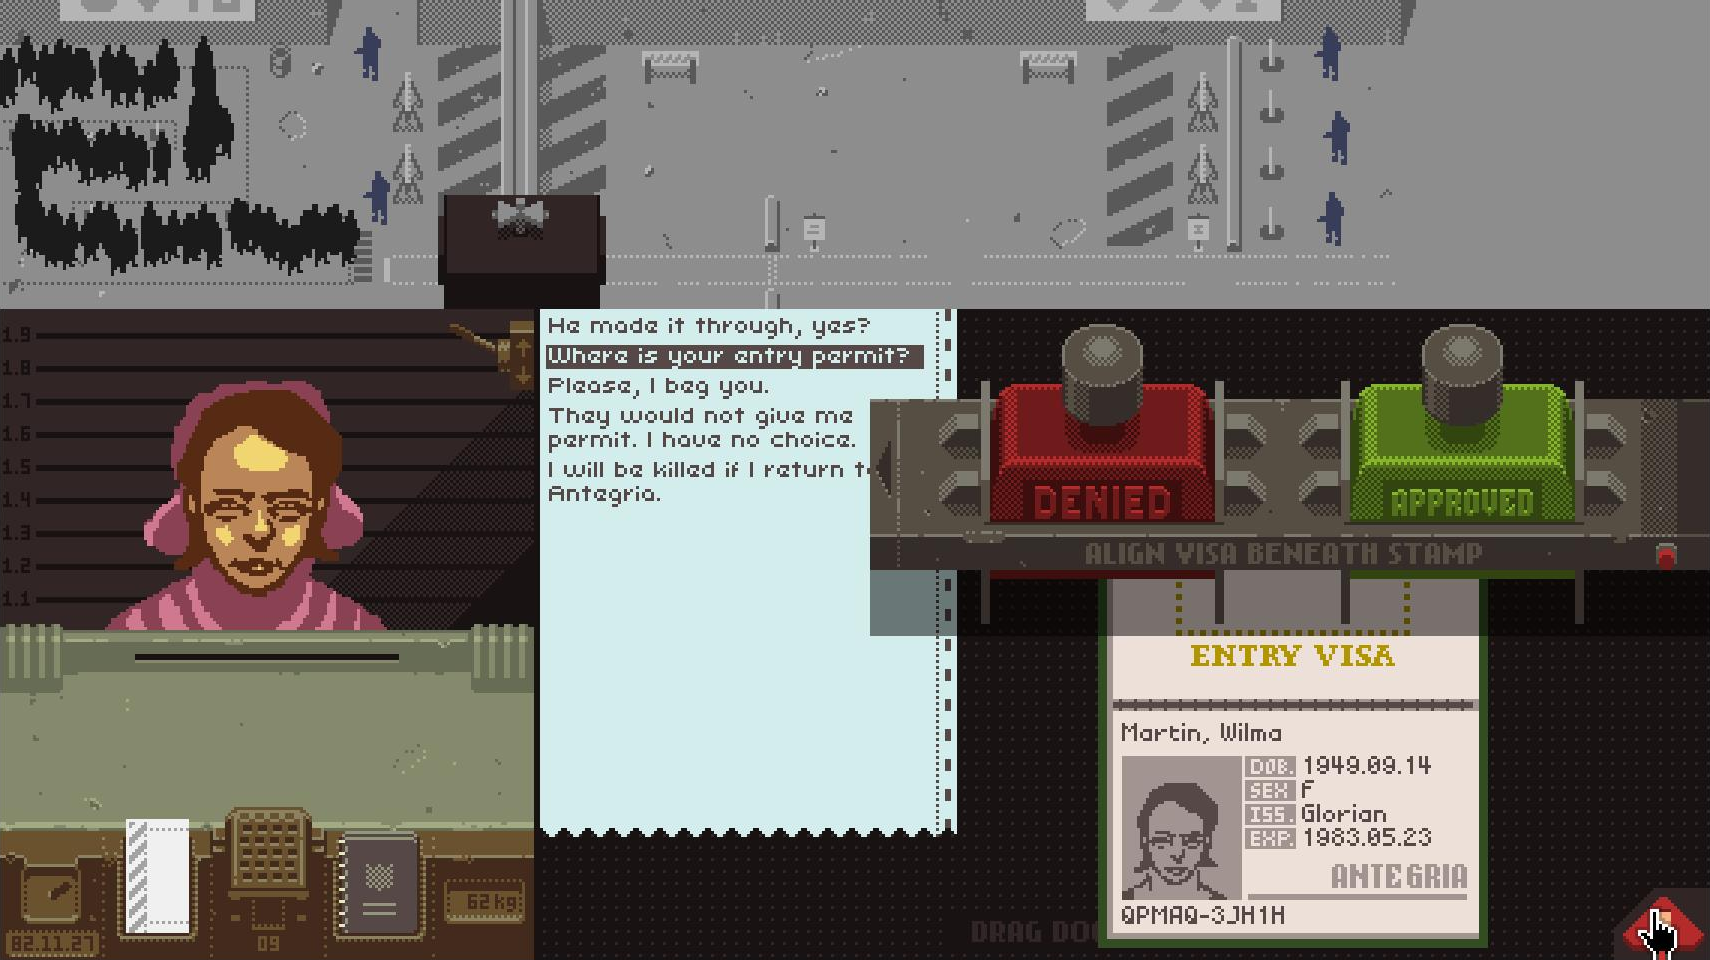
\includegraphics[width=\textwidth]{fig/papers-please-visa-choice.png}
  \caption{A screenshot from \DIFdelbeginFL \emph{\DIFdelFL{Papers Please}} %DIFAUXCMD
\DIFdelendFL \DIFaddbeginFL \emph{\DIFaddFL{Papers, Please}} \DIFaddendFL showing the interface as the player decides whether or not to admit a traveler. The traveler in question claims that she was denied an entry permit but will be killed if turned away. At this point, the player may pursue further questioning or examine the details of the applicant's passport, but must eventually either approve or deny her entry visa.}
  \label{fig:PP_visa}
\end{figure}



\DIFdelbegin %DIFDELCMD < \section{Uncertainty and Complicity in \emph{Papers Please}}
%DIFDELCMD < %%%
\DIFdelend \DIFaddbegin \section{Uncertainty and Complicity in \emph{Papers, Please}}
\DIFaddend 

\emph{Papers\DIFaddbegin \DIFadd{, }\DIFaddend Please} \citep{pope2013papers} gives the player the role of a border inspector in the fictional autocratic regime of Arstotzka.
%
Struggling to support their family at home, they are challenged to quickly inspect passports, visas, and eventually travel permits and vaccination records to either permit or deny entry for a stream of hopeful immigrants and travelers, earning money for each applicant correctly approved or denied.
%
A central part of the game is unresolved ambiguity, both about the identities and claims of those seeking entry and about the motives and legitimacy of the government and opposing revolutionary forces.
%
\cite{alexander2013designing} gives a nice overview of the game from a critical perspective, and \cite{formosa2016papers} provides a detailed analysis of its systemic engagement with a variety of moral issues.


Of interest to this analysis is the choice shown in Fig \ref{fig:PP_visa}, which comes up in several different guises throughout the game.
%
In each case, the player must decide whether to take someone at their word that despite a missing or incorrect document, they deserve admission because they would face terrible consequences were they refused.
%
This decision is complicated by the fact that the game also presents situations where \DIFdelbegin \DIFdel{entrants }\DIFdelend \DIFaddbegin \DIFadd{applicants }\DIFaddend attempt to bribe or threaten the player, implying that not all of their claims can be taken at face value.
%
This decision about the fate of an ostensible refugee embodies one of the central themes of the game: how the uncertainty of information from unreliable sources can be pitted against the certain plight of one's family to turn a moral dilemma into a choice with a reluctant ``better'' option.
%
In the rest of this section, we show the results of each step of a choice poetic analysis (see section \ref{sec:analysis_steps}) for the choice described in Fig. \ref{fig:PP_visa}.

\subsection{Goal Analysis}

For the purposes of understanding this choice, it is sufficient to use a single player model with the following prioritized goals:
\begin{itemize}
  \item (high-priority) Provide for your family---the player wants to earn credits and avoid penalties to be able to pay for food and shelter at the end of the day.
  \item (high-priority) Act ethically---as much as possible, the player wants to treat applicants ethically and avoid acting in ways that would intentionally harm them without reason, even when this goes against the government's dictates.
  \item (medium-priority) Apprehend criminals---separate from their desire to earn credits, the player actively wants to identify applicants who might be attempting to gain entry to the country deceitfully and reject their applications.
  \item (low-priority) Admit approved travellers---all else being equal, the player seeks to treat applicants fairly and admit those that have everything in order.
\end{itemize}
If we were concerned about differences between players, we could repeat this analysis with another set of player goals and contrast the results, as we did with \emph{Undertale}.
%DIF > 
\DIFaddbegin \DIFadd{Note that especially in this case, the results of the analysis inform and justify the player model used.
%DIF > 
If results differ significantly from what we know about a choice, there are two possibilities: either one or more of our assumptions (about goals, goal priorities, and/or the perception of outcomes) was wrong, in which case we can revise or extend our assumptions and re-do the analysis, or what we thought we knew was wrong, and we should be able to use our analysis to demonstrate why.
%DIF > 
In this case, we think, based on other analyses and interviews with the game designer, that }\emph{\DIFadd{Papers, Please}} \DIFadd{uses ambiguity to encourage complicity, and through a formal analysis, we should be able to either back up that intuition or demonstrate why things do not actually work that way.
}\DIFaddend 


\DIFaddbegin \DIFadd{Because choice poetics makes its assumptions about player motivations and perceived outcome likelihoods explicit these aspects of the analysis can be easily examined and criticized.
%DIF > 
In many cases, the most efficient means of dealing with such criticism is to expand the analysis or contrast it with a proposed alternative.
%DIF > 
When an analysis disagrees with other sources, the source of that disagreement is often differing assumptions about how players will perceive a choice or about how they will respond to the options offered.
%DIF > 
Making those assumptions explicit thus helps ground potential disagreements, and not only allows for stating disagreements clearly (e.g., ``I don't think that most players will place a high priority on acting ethically.'') but allows for alternative assumptions to be tested using an identical analytical process.
}


\DIFadd{When an analysis agrees with other sources in its conclusions, the burden is on the critic to argue why a specific choice of goal priorities or outcome likelihoods is unrealistic, and demonstrate how that affects the overall argument put forward.
%DIF > 
Ideally, of course, such questions might also be settled by gathering real data about player perceptions of goals and outcomes, and choice poetics provides a framework for doing so (see \mbox{%DIFAUXCMD
\cite{mawhorter2015intentionally}}\hspace{0pt}%DIFAUXCMD
).
}

\DIFaddend \begin{table}[H]
\centering
\begin{tabular}{l l}
  \toprule
  \multicolumn{1}{c}{\textbf{Approve}} & \multicolumn{1}{c}{\textbf{Deny}} \\
  \midrule
  (likely) Don't earn a credit & (likely) Earn a credit \\
  (likely) Get punished & (likely) No punishment \\
  (unknown) Refugee is saved & (unknown) Refugee is condemned \\
  (unknown) Scam is rewarded & (unknown) Scam is thwarted \\
  \bottomrule
\end{tabular}
\DIFdelbeginFL %DIFDELCMD < \caption[\emph{Papers Please} likelihood analysis]{%%%
\DIFdelendFL \DIFaddbeginFL \caption[\emph{Papers, Please} likelihood analysis]{\DIFaddendFL Likelihood analysis for the choice shown in Fig. \ref{fig:PP_visa}.}
\label{tab:PP_likelihoods}
\end{table}

\subsection{Likelihood Analysis}

Table \ref{tab:PP_likelihoods} shows a breakdown of outcomes and their likelihoods for both possible decisions; relevant outcomes have been essentially intuited from player goals.
%
Note in particular the outcomes with unknown likelihood that represent competing possible worlds with respect to the trustworthiness of the applicant: if they are telling the truth about their plight, admitting them realizes a different outcome than if they are just making up their story to gain entrance, and the player does not have enough information to make an informed judgement either way.


\begin{table}[H]
\centering
\begin{tabular}{c l l l l l}
  \toprule
  & \multicolumn{2}{c}{\textbf{With Suspicion}} && \multicolumn{2}{c}{\textbf{Without Suspicion}} \\
  \cmidrule(r){1-1} \cmidrule{2-3} \cmidrule{5-6}
  \textbf{Goal} & \multicolumn{1}{c}{\textbf{Approve}} & \multicolumn{1}{c}{\textbf{Deny}} && \multicolumn{1}{c}{\textbf{Approve}} & \multicolumn{1}{c}{\textbf{Deny}} \\
  \cmidrule(r){1-1} \cmidrule{2-3} \cmidrule{5-6}
  \multirow{2}{9em}{\centering provide-for-family} & \threatens{} & \enables{} && \threatens{} & \enables{} \\
                                        & \hinders{} & \advances{} && \hinders{} & \advances{} \\
  \cmidrule(r){1-1} \cmidrule{2-3} \cmidrule{5-6}
  \multirow{2}{9em}{\centering act-ethically} & \multirow{2}{6em}{\enables{}} & \multirow{2}{6em}{\threatens{}} && \enables{} & \threatens{} \\
  & & && \advances{} & \hinders{} \\
  \cmidrule(r){1-1} \cmidrule{2-3} \cmidrule{5-6}
  apprehend-criminals & \threatens{} & \enables{} && <none> & <none> \\
  \cmidrule(r){1-1} \cmidrule{2-3} \cmidrule{5-6}
  admit-approved & <none> & <none> && <none> & <none> \\
  \bottomrule
\end{tabular}
  \DIFdelbeginFL %DIFDELCMD < \caption[\emph{Papers Please} option analysis]{%%%
\DIFdelendFL \DIFaddbeginFL \caption[\emph{Papers, Please} option analysis]{\DIFaddendFL Option analysis for the example choice shown in Fig. \ref{fig:PP_visa}. The default analysis is shown on the left (`With Suspicion'), and a revised analysis assuming that the player trusts the applicant (`Without Suspicion') is shown on the right. See section \ref{sec:prospective_labels} for how the labels were applied.}
\label{tab:PP_options}
\end{table}

\subsection{Prospective Analysis}

The prospective analysis results are shown on the left side of Table \ref{tab:PP_options}; note that one of the goals (that of admitting approved applicants) is irrelevant here.
%
From these results, we can immediately see that although both options threaten some goals, the deny option is clearly better with regards to the high-priority goal of feeding your family.
%
In fact, although approving the applicant \emph{might} be an ethical action, that is not certain, and denying the applicant might also be in line with \DIFaddbegin \DIFadd{our player model's }\DIFaddend ethical standards if in fact they are making up their story.


While this choice does not contain any well-known outcome patterns (cf. \cite{mawhorter2014towards}), it does involve some moral concerns, pitting one's desire to help one's family against concerns about turning away a refugee.
%
The structure is clarified further if we consider the same analysis under the assumption that the applicant is telling the truth, which is shown on the right side of Table \ref{tab:PP_options}.
%
This new analysis has the structure of a classic dilemma: Two options, each of which \hinders{} an equally important goal.
%
Compared to the left side of Table \ref{tab:PP_options}, concerns about apprehending criminals are gone, and the refugee-related outcomes, now believed to be likely, make the moral weight of the decision unambiguous.


This comparison thus illustrates exactly how \emph{Papers\DIFaddbegin \DIFadd{, }\DIFaddend Please} (and governments) can manufacture complicity: by introducing doubts about the motives of strangers while emphasizing the certainty of outcomes for loved ones, a dilemma that clearly warrants serious moral concern can be transformed into an uneven choice where multiple avenues of justification are available.
%
Note in particular that the \DIFdelbegin \DIFdel{model player }\DIFdelend \DIFaddbegin \DIFadd{player model}\DIFaddend 's goal of apprehending criminals was not a deciding factor in this case.
%
Regardless of the existence of that goal, uncertainty about the applicant's situation still eliminates any \advances{} labels from the `Approve' column while leaving the `Deny' column \hinders{}-free.
%
The ambiguous decision is still not an easy one, as evidenced by the fact that it \threatens{} a top-priority goal (behaving ethically).
%
This leaves the player feeling uneasy about the decision, and potentially helps prompt more reflection on the decision, but ultimately our \DIFdelbegin \DIFdel{model player }\DIFdelend \DIFaddbegin \DIFadd{player model }\DIFaddend will still view denying the application as the better choice once uncertainty is introduced.

\subsection{Retrospective Analysis}

At the end of each day in \emph{Papers\DIFaddbegin \DIFadd{, }\DIFaddend Please}, the player is paid based on the number of applicants they processed ``correctly,'' and then must decide how much money to allocate for family needs, such as food, heating, and eventually, medicine.
%
However, except in a few special cases, there is no information provided about the subsequent outcomes for the applicants who have entered the country that day.
%
\DIFaddbegin \DIFadd{In cases where information is available, it is as likely to raise more suspicions as assuage them: }\DIFaddend The player is \DIFaddbegin \DIFadd{eventually asked to participate in a plot to overthrow the Arstotzkan government, and both sides of the conflict are presented as having questionable motives.
%DIF > 
The player is }\DIFaddend thus not given \DIFdelbegin \DIFdel{a chance to form any kind of justification for }\DIFdelend \DIFaddbegin \DIFadd{many chances to justify }\DIFaddend their beliefs about the truth of applicants' statements\DIFaddbegin \DIFadd{, and in some cases, is given extra reasons to doubt them}\DIFaddend .
%
Of course, such blanket beliefs about future applicants based on past applicants are simple biases, not rational conclusions, because the applicants are independent of each other, but they would help assuage the player's conscience (or potentially inflame it if the evidence contradicted the player's assumptions).
%
However, by denying even such a false sense of closure, the game encourages the player to feel vaguely uneasy about their role.



At the same time, by emphasizing the outcomes for the player's family, the game pushes the player away from the dilemma mindset and towards an obvious justification for complicity: the player ``had'' to act in the state's interests because their family's welfare was at stake.
%
From a choice poetic perspective, this choice thus has two interesting properties: First, certain outcomes remain hidden from the player indefinitely, and second, the outcomes that are apparent are emphasized in the course of continued play.
%
The withholding of information serves the purpose of introducing and even emphasizing the uncertainty about outcomes that tilts the choice as discussed above, while the emphasis on the relatively certain outcomes gives the player an extra push towards viewing the choice not as a moral dilemma but as a situation where there is only one ``correct'' choice.

\DIFaddbegin \subsection{Discussion}

\DIFadd{As with our }\emph{\DIFadd{Undertale}} \DIFadd{analysis, the conclusions we reach are the same as those of other analysts \mbox{%DIFAUXCMD
\citep{alexander2013designing,formosa2016papers}}\hspace{0pt}%DIFAUXCMD
, which is encouraging, because it validates our methodology.
%DIF > 
At the same time, the level of detail we achieve enables us to answer further questions: }\emph{\DIFadd{how}} \DIFadd{exactly does ambiguity play a role in encouraging complicity in }\emph{\DIFadd{Papers, Please}}\DIFadd{, and }\emph{\DIFadd{what}} \DIFadd{changes in player mindset or choice specifics might lead to a different outcome?
}


\DIFadd{Having set out to understand how exactly }\emph{\DIFadd{Papers, Please}} \DIFadd{uses ambiguity to encourage complicity, we have used choice poetics to provide a detailed explanation of the mechanisms behind this effect.
%DIF > 
The comparison presented in Table \ref{tab:PP_options} shows that suspicion about the motives of petitioners is key to turning a dilemma into a more murky and lopsided choice.
%DIF > 
From this detailed analysis, we can also see which aspects of the player's mindset are necessary for this effect to occur: The player model's goal of apprehending criminals is surprisingly irrelevant to the deconstruction of the dilemma, because the goal of providing for one's family pushes in the same direction and is more clearly established by the context of the decision.
%DIF > 
What is important instead is the player's willingness to be persuaded that some applicants do not deserve entry, and that denying them entry would be a good thing.
%DIF > 
An anarchist player who believed that denying anyone entry was immoral (or at least, that some balance of honest and dishonest applicants should always be resolved to favor the honest applicants) would resist the technique used here and face a clear dilemma between feeding their family and obeying their conscience.
}


\DIFaddend \section{Conclusion}

Through our analyses of \DIFdelbegin \emph{\DIFdel{Mass Effect}}%DIFAUXCMD
\DIFdel{, }\DIFdelend \DIFaddbegin \DIFadd{choices from }\DIFaddend \emph{Undertale} \DIFdelbegin \DIFdel{, and }\DIFdelend \DIFaddbegin \DIFadd{and }\DIFaddend \emph{Papers\DIFaddbegin \DIFadd{, }\DIFaddend Please}, we have demonstrated the concrete application of choice poetics to \DIFdelbegin \DIFdel{three }\DIFdelend \DIFaddbegin \DIFadd{two }\DIFaddend very different choices\DIFdelbegin \DIFdel{, and hopefully the framework's utility is evident from the conclusions we have drawn}\DIFdelend .
%
\DIFdelbegin \DIFdel{Certainly, as }\DIFdelend \DIFaddbegin \DIFadd{As }\DIFaddend already mentioned, the \DIFdelbegin \DIFdel{statements made }\DIFdelend \DIFaddbegin \DIFadd{conclusions drawn }\DIFaddend here about both games have already been \DIFdelbegin \DIFdel{made to some degree }\DIFdelend \DIFaddbegin \DIFadd{reached }\DIFaddend by others, \DIFdelbegin \DIFdel{and choice poetics does not claim to generate insights that are radically different from those drawn by experienced games critics}\DIFdelend \DIFaddbegin \DIFadd{which confirms that our analytical approach leads to sound conclusions}\DIFaddend .
%
\DIFdelbegin \DIFdel{Instead}\DIFdelend \DIFaddbegin \DIFadd{Relative to a typical close reading approach}\DIFaddend , choice poetics \DIFdelbegin \DIFdel{has three goals: first, to provide a }\emph{\DIFdel{computable}} %DIFAUXCMD
\DIFdel{framework for automated reasoning about choices (as discussed in previous literature) , second to make that framework accessible to critics (especially novice critics) so that they can systemically }\DIFdelend \DIFaddbegin \DIFadd{provides extra formal structure that encourages detailed observation and which can lead to secondary observations about the choice being analyzed.
%DIF > 
In addition, where a close reading uses the author's experience to stand in for the experience of players, choice poetics forces the analyst to create explicit player models, thus reifying their assumptions about how choices will be perceived and opening them up for examination.
%DIF > 
The assumptions that choice poetics makes about player goals are thus both a weakness (they might be wrong) and a strength (errors can be identified exactly, and contrasting analyses can test hypotheses about player goals).
}


\DIFadd{Besides encouraging more explicit examination of choices, we also hope that a formalist framework can make analysis more accessible to novice critics, allowing them to systematically }\DIFaddend identify interesting aspects of a choice, and \DIFdelbegin \DIFdel{third, to provide a detailed language for talking about narrative choices to aid precise communication about }\DIFdelend \DIFaddbegin \DIFadd{that it can provide precise language for describing narrative choices and }\DIFaddend their poetic effects\DIFdelbegin \DIFdel{, as well as precise reasoning about what changes might be made to achieve different effects}\DIFdelend .
%
Ideally, choice poetics should support discussions about why and how a choice achieves its poetic effect, and should enable those discussions to be more detailed and specific.


\DIFdelbegin \DIFdel{In our analysis of }\emph{\DIFdel{Mass Effect}}%DIFAUXCMD
\DIFdel{, we demonstrated how the theory's emphasis on }\DIFdelend \DIFaddbegin \DIFadd{To explore }\DIFaddend modes of engagement\DIFdelbegin \DIFdel{naturally leads to the question: ``If this choice doesn't }\emph{\DIFdel{seem}} %DIFAUXCMD
\DIFdel{to have any relevant outcomes, for what kind of player (i.e., for what set of player goals) would it be relevant?''
%DIF < 
From there, we found that although some of }\emph{\DIFdel{Mass Effect}}%DIFAUXCMD
\DIFdel{'s choices have no mechanical or diegetic differences between outcomes, from a narrative perspective they can change the player's (or a spectator's) interpretation of a character, and that is enough to be meaningful to some players.
%DIF < 
Ultimately, this analysis highlights the importance of considering player motives when analyzing choices, and also foregrounds how broad the notion of a `consequence' is in narrative games.
}%DIFDELCMD < 

%DIFDELCMD < %%%
\DIFdel{Furthering our exploration of modes of engagement, we }\DIFdelend \DIFaddbegin \DIFadd{, we }\DIFaddend gave an example of paired choice analysis with \DIFaddbegin \DIFadd{a central and recurring choice from }\DIFaddend \emph{Undertale}, showing how choice poetics can be used to contrast different play styles.
%
The benefit in this case was a detailed look at how \emph{Undertale} separates players with different priorities into different choice patterns in order to encourage dialogue between players who experience the game differently, including how divergence is encouraged at both initial and subsequent encounters with a repeated choice.
%
Choice poetics helps pinpoint exactly which outcomes drive that separation, and what sets of priorities are necessary for it to happen.


We then went into depth with \emph{Papers\DIFaddbegin \DIFadd{, }\DIFaddend Please}, using prospective and retrospective analysis to pin down subtle characteristics of a common choice in that game.
%
Noting how uncertainty undermined a dilemma configuration for that choice, we were able to describe in detail how that choice tilts players towards complicity with the game's fictional regime, and what other aspects of the choice design help contribute to this outcome.
%
In fact, our analysis reveals several simple changes that could have been implemented had the author wished to create a different narrative.
%
For example, revealing after-the-fact that most applicants begging for asylum were in fact refugees would be enough to permit a story where the player bravely resists their regime's authoritarian tendencies by turning the present ambiguous choice into a clear moral dilemma.
%
The utility of choice poetics here then is to identify exactly how a choice creates a certain feeling, and which elements of the choice might be changed to create a different one.


In all of the analyses presented here, we engage with choice poetics as human scholars, using only those pieces of the theory that are relevant to the specific choices at hand and glossing over details that seem evident from common sense.
%
Although choice poetics was designed with operationalization in mind, our analyses show that it can also be of use to human critics as a framework for discussion.
%
We also expect that the framework's systematic steps will be useful when confronted with choices that are difficult to understand, and that the notion of different \DIFdelbegin \DIFdel{model players }\DIFdelend \DIFaddbegin \DIFadd{player models }\DIFaddend will help illuminate choices that leave different actual players feeling different things.


As we continue to develop this theory, we plan to explore further computational models and collect and analyze play traces to demonstrate the theory's utility in the domain of automated analysis, with the eventual goal of using it for on-line player modelling to enable responsive stories.
%
Additionally, we hope to remain in dialogue with critics and games scholars who seek to understand narrative choices, and hope that our framework can at least provide useful language to this community for discussing poetic choices.
%
Of course, we will also continue examining games, and may come up with more examples of how choice poetics can be productively applied to understanding how their choices fit into their narratives.

%%%%%%%%%%%%%%%%%%%%%%%%%%%%%%%%%%%%%%%%%%
\vspace{6pt} 

% Supplementary material
\DIFdelbegin %DIFDELCMD < \supplementary{A video illustrating the possible outcomes of one false choice in \emph{Mass Effect} is available at \linksupplementary{s1}, as well as on YouTube at \url{https://www.youtube.com/watch?v=8BewZnUnDoE}.}
%DIFDELCMD < %%%
\DIFdelend \DIFaddbegin \supplementary{None.}
\DIFaddend 

%%%%%%%%%%%%%%%%%%%%%%%%%%%%%%%%%%%%%%%%%%
\authorcontributions{Conceptualization, all authors; Investigation, Peter Mawhorter, Carmen Zegura, Alex Gray, and Arnav Jhala; Writing--Original Draft Preparation, Peter Mawhorter, Carmen Zegura, and Alex Gray; Writing--Review \& Editing, Peter Mawhorter and Noah Wardrip-Fruin.}

%%%%%%%%%%%%%%%%%%%%%%%%%%%%%%%%%%%%%%%%%%
\funding{The authors would like to acknowledge the support of NSF grant IIS-1409992, which supported some of the initial development of choice poetics.}

%%%%%%%%%%%%%%%%%%%%%%%%%%%%%%%%%%%%%%%%%%
\conflictsofinterest{The authors declare no conflict of interest.}

%%%%%%%%%%%%%%%%%%%%%%%%%%%%%%%%%%%%%%%%%%
\externalbibliography{yes}
\bibliography{references}

\end{document}
